%%%%%%%%%%%%%%%%%%%%%%%%%%%%%%%%%%%%%%%%%
% Beamer Presentation
% LaTeX Template
% Version 1.0 (10/11/12)
%
% This template has been downloaded from:
% http://www.LaTeXTemplates.com
%
% License:
% CC BY-NC-SA 3.0 (http://creativecommons.org/licenses/by-nc-sa/3.0/)
%
%%%%%%%%%%%%%%%%%%%%%%%%%%%%%%%%%%%%%%%%%

%----------------------------------------------------------------------------------------
%	PACKAGES AND THEMES
%----------------------------------------------------------------------------------------

\documentclass{beamer}

\mode<presentation> {

% The Beamer class comes with a number of default slide themes
% which change the colors and layouts of slides. Below this is a list
% of all the themes, uncomment each in turn to see what they look like.

%\usetheme{default}
%\usetheme{AnnArbor}
%\usetheme{Antibes}
%\usetheme{Bergen}
%\usetheme{Berkeley}
%\usetheme{Berlin}
%\usetheme{Boadilla}
%\usetheme{CambridgeUS}
%\usetheme{Copenhagen}
%\usetheme{Darmstadt}
%\usetheme{Dresden}
%\usetheme{Frankfurt}
%\usetheme{Goettingen}
%\usetheme{Hannover}
%\usetheme{Ilmenau}
%\usetheme{JuanLesPins}
%\usetheme{Luebeck}
\usetheme{Madrid}
%\usetheme{Malmoe}
%\usetheme{Marburg}
%\usetheme{Montpellier}
%\usetheme{PaloAlto}
%\usetheme{Pittsburgh}
%\usetheme{Rochester}
%\usetheme{Singapore}
%\usetheme{Szeged}
%\usetheme{Warsaw}

% As well as themes, the Beamer class has a number of color themes
% for any slide theme. Uncomment each of these in turn to see how it
% changes the colors of your current slide theme.

%\usecolortheme{albatross}
%\usecolortheme{beaver}
%\usecolortheme{beetle}
%\usecolortheme{crane}
%\usecolortheme{dolphin}
%\usecolortheme{dove}
%\usecolortheme{fly}
%\usecolortheme{lily}
%\usecolortheme{orchid}
%\usecolortheme{rose}
%\usecolortheme{seagull}
%\usecolortheme{seahorse}
%\usecolortheme{whale}
%\usecolortheme{wolverine}

%\setbeamertemplate{footline} % To remove the footer line in all slides uncomment this line
%\setbeamertemplate{footline}[page number] % To replace the footer line in all slides with a simple slide count uncomment this line

%\setbeamertemplate{navigation symbols}{} % To remove the navigation symbols from the bottom of all slides uncomment this line
}


\usepackage{booktabs} % Allows the use of \toprule, \midrule and \bottomrule in tables
\usepackage{listings}

\usepackage{minted}
\usepackage[utf8]{inputenc}
\usepackage[T2A]{fontenc}
\usepackage{amssymb, amsmath, mathrsfs, amsthm}
\usepackage[russian]{babel}
\usepackage{float}
\usepackage{pgfplotstable}
\usepackage{multirow}
\graphicspath{{./}}

%----------------------------------------------------------------------------------------
%	TITLE PAGE
%----------------------------------------------------------------------------------------

\title[Визуализация данных]{Визуализация данных} % The short title appears at the bottom of every slide, the full title is only on the title page

\author[Попов Дмитрий]{Попов Дмитрий Олегович} % Your name
\institute[МГУ, ВМК]{Московский государственный университет имени М.В. Ломоносова\\
Факультет вычислительной математики и кибернетики\\
Кафедра математических методов прогнозирования\\
~\\
\textbf {Творческое домашнее задание 1}\\
~\\
Прикладные задачи анализа данных
} % Your institution as it will appear on the bottom of every slide, may be shorthand to save space
{
\medskip
}
\date{\today} % Date, can be changed to a custom date

\begin{document}

\begin{frame}
\titlepage % Print the title page as the first slide
\end{frame}

%----------------------------------------------------------------------------------------
%	PRESENTATION SLIDES
%----------------------------------------------------------------------------------------

\begin{frame}{Набор данных}

https://www.kaggle.com/ruchi798/malnutrition-across-the-globe\\

Выложен полгода назад.\\

Данные об исследованиях пяти параметров в странах по всему миру с 1983 по 2019 год.\\

10 ноутбуков, где-то 3 из них посвящены визуализации данных.


\end{frame}

\begin{frame}{Какие данные доступны}

Объектом в выборке данных является исследование.\\

Пять ординальных переменных, которые я интерпретирую как признаки: группа уровня дохода, наименее развитые страны, низкий доход/недостаток пищи в стране, неразвитая страна без выхода к морю, неразвитая страна на малом острове.\\
Дополнительные признаки: год, количество исследований по стране, страна.\\

Пять действительных переменных: недовес, истощение, сильное истощение, низкорослость, избыток веса.

\end{frame}

\begin{frame}

\begin{figure}
	\centering
	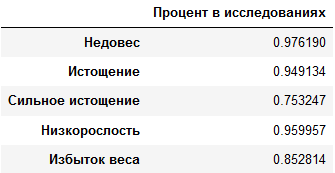
\includegraphics[width=60mm]{1.png}
\end{figure}


\end{frame}

\begin{frame}

\begin{figure}
	\centering
	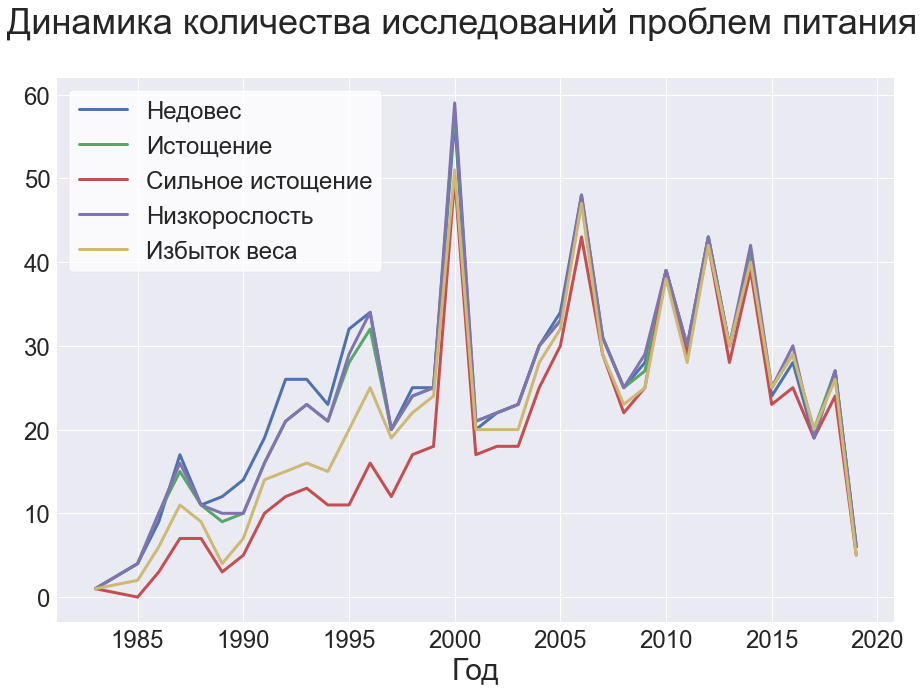
\includegraphics[width=100mm]{2.png}
\end{figure}


\end{frame}



\begin{frame}

\begin{figure}
	\centering
	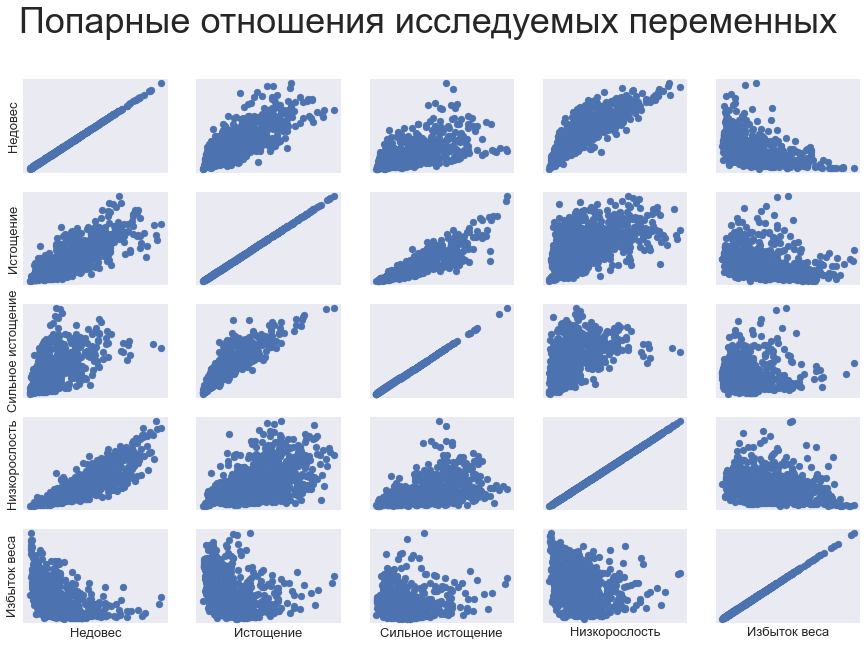
\includegraphics[width=100mm]{3.png}
\end{figure}


\end{frame}



\begin{frame}

\begin{figure}
	\centering
	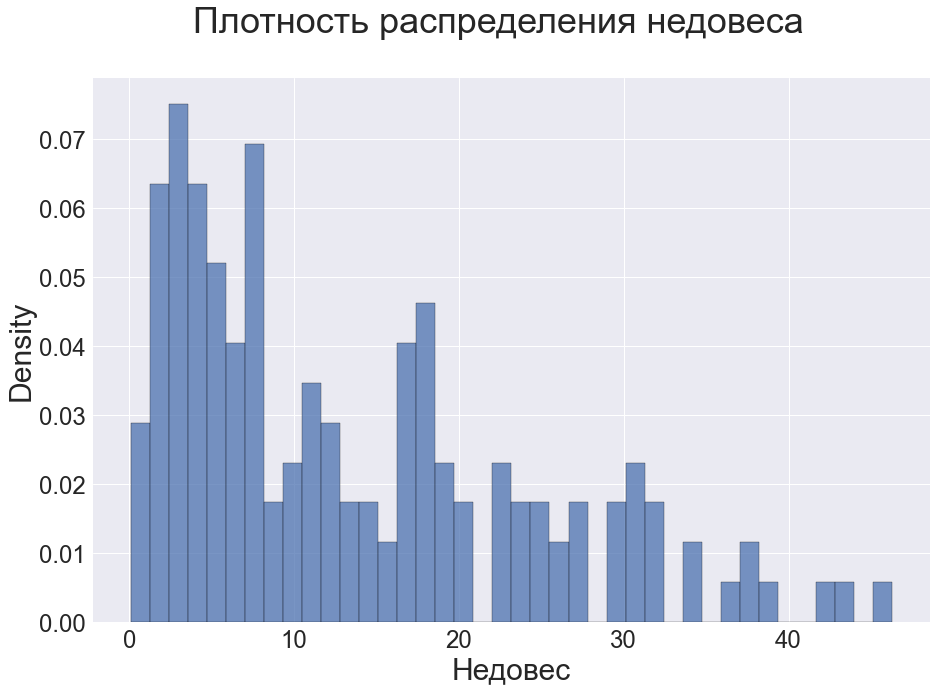
\includegraphics[width=120mm]{4.png}
\end{figure}


\end{frame}



\begin{frame}

\begin{figure}
	\centering
	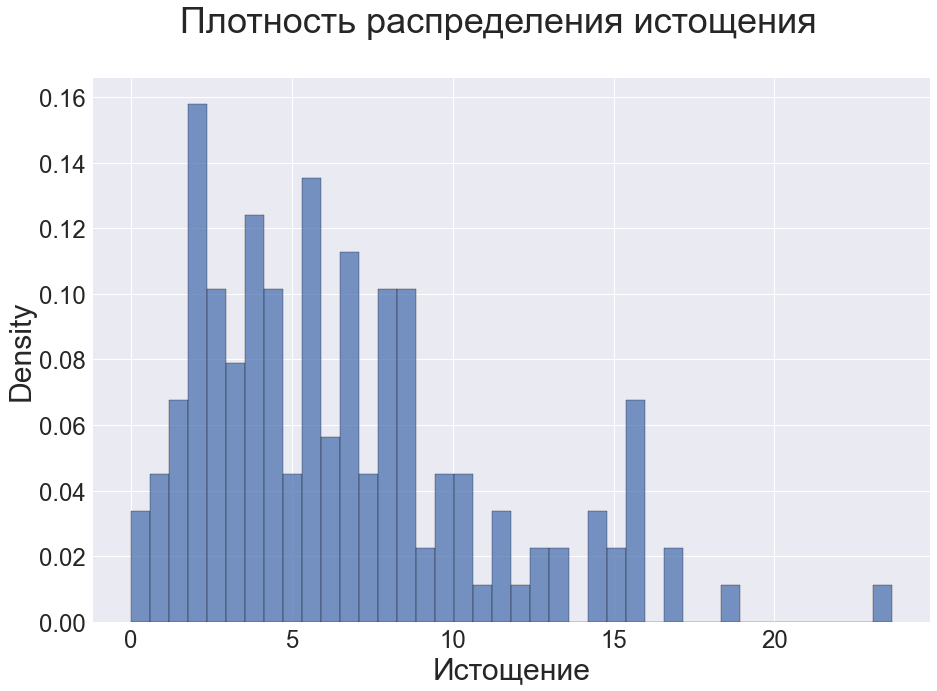
\includegraphics[width=120mm]{5.png}
\end{figure}


\end{frame}



\begin{frame}

\begin{figure}
	\centering
	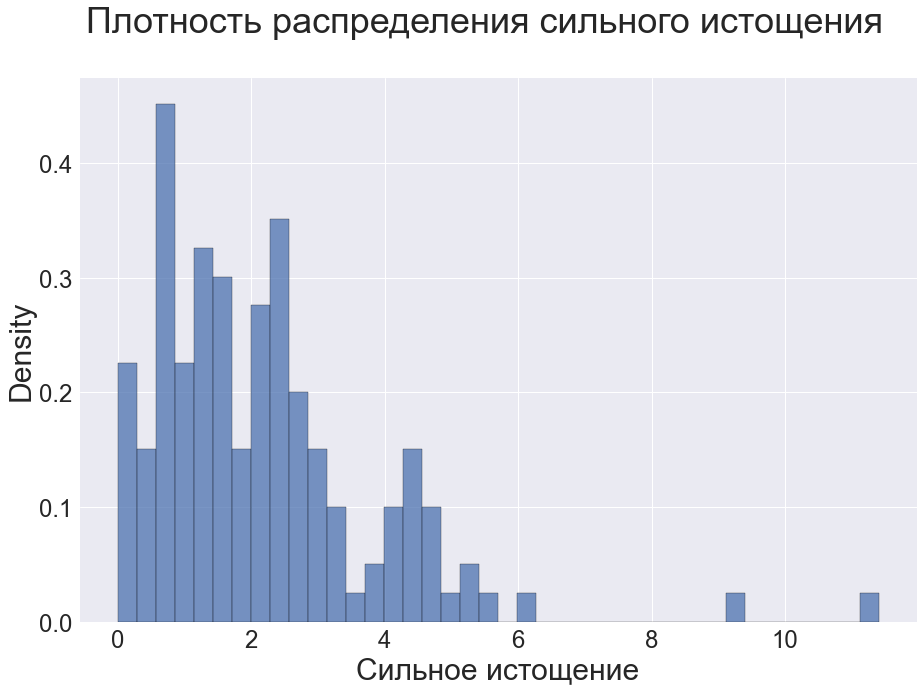
\includegraphics[width=120mm]{6.png}
\end{figure}


\end{frame}



\begin{frame}

\begin{figure}
	\centering
	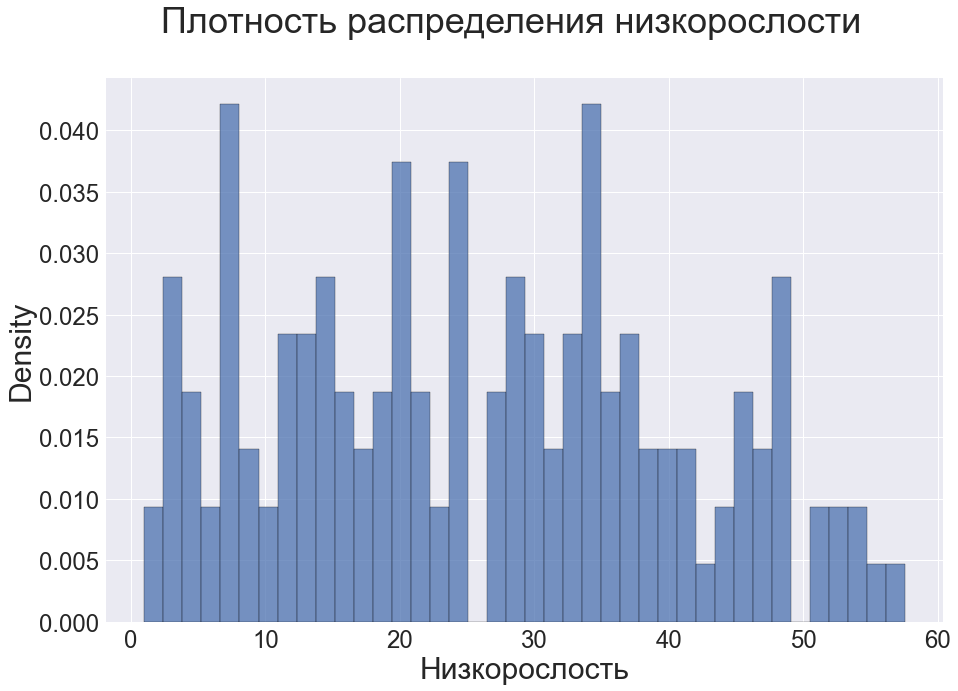
\includegraphics[width=120mm]{7.png}
\end{figure}


\end{frame}



\begin{frame}

\begin{figure}
	\centering
	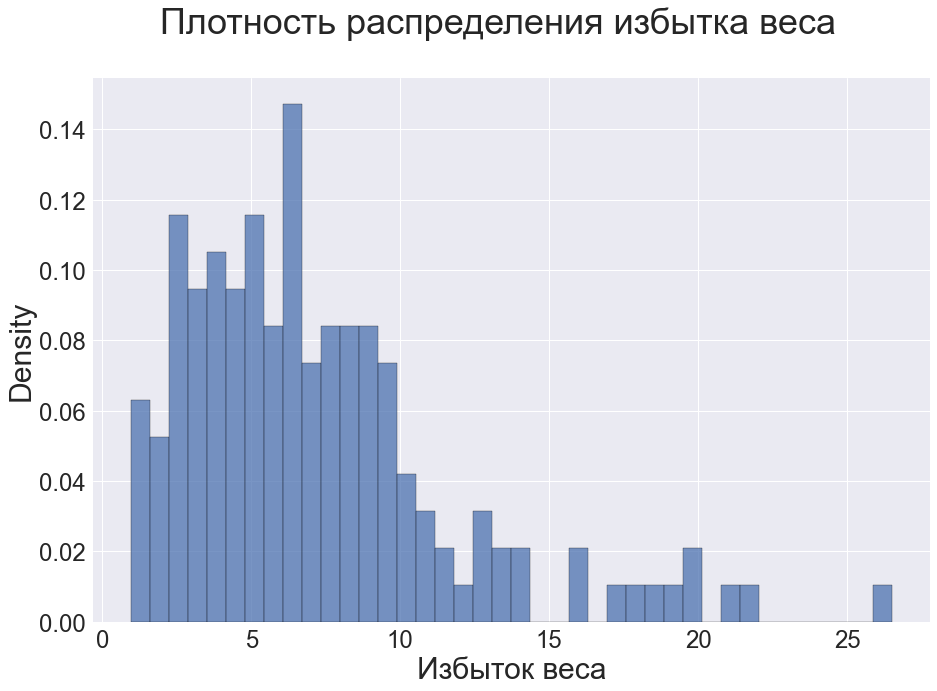
\includegraphics[width=120mm]{8.png}
\end{figure}


\end{frame}



\begin{frame}

\begin{figure}
	\centering
	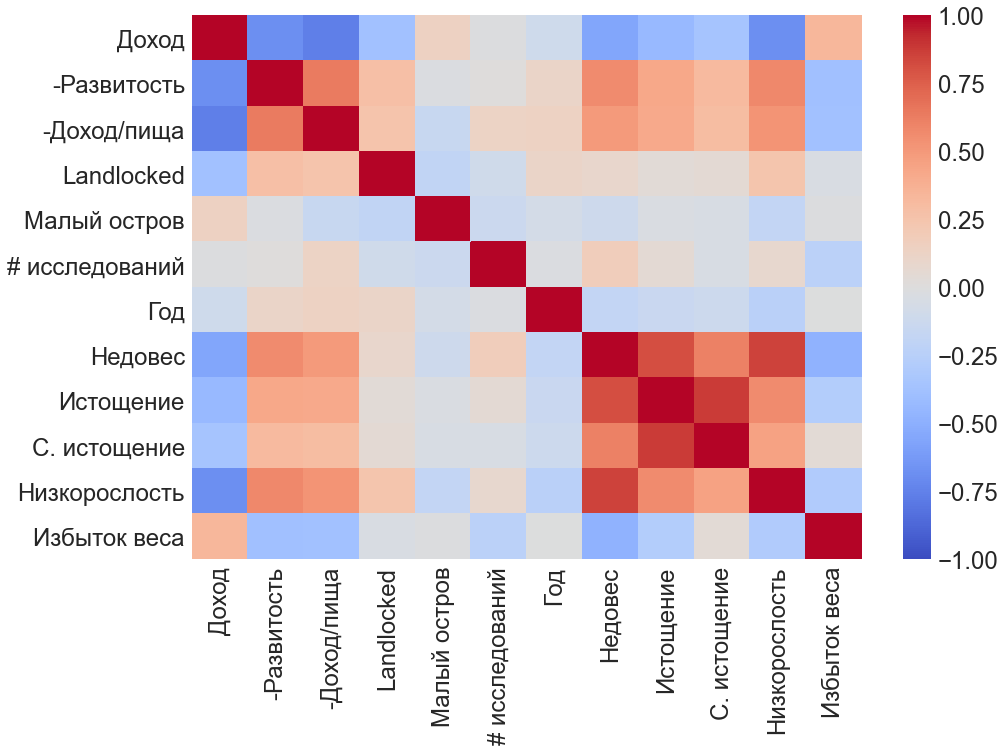
\includegraphics[width=120mm]{9.png}
\end{figure}


\end{frame}


\begin{frame}

\begin{figure}
	\centering
	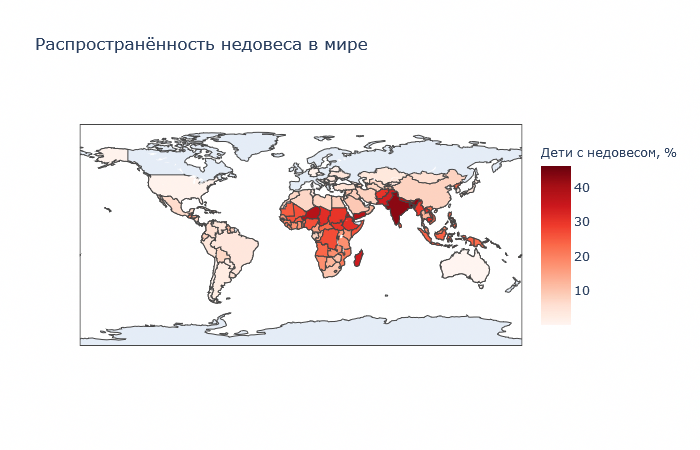
\includegraphics[width=125mm]{10.png}
\end{figure}


\end{frame}


\begin{frame}

\begin{figure}
	\centering
	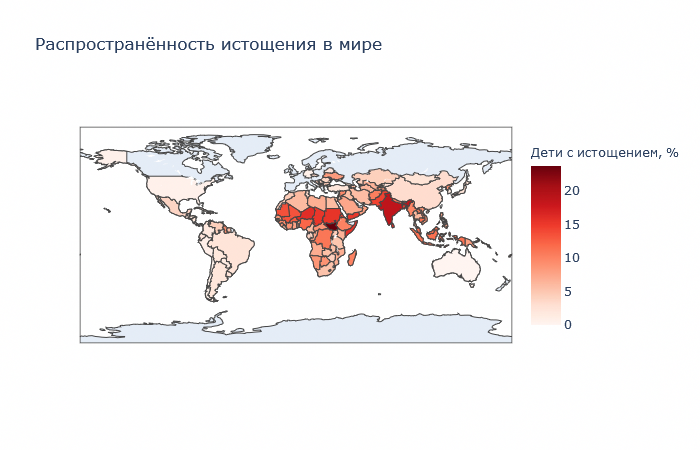
\includegraphics[width=125mm]{11.png}
\end{figure}


\end{frame}


\begin{frame}

\begin{figure}
	\centering
	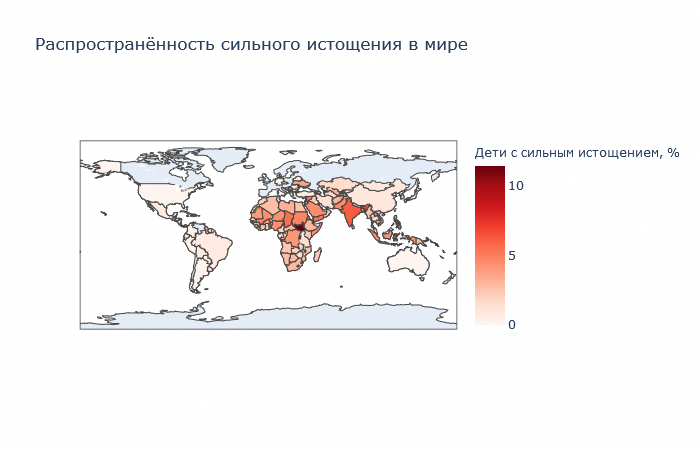
\includegraphics[width=125mm]{12.png}
\end{figure}


\end{frame}


\begin{frame}

\begin{figure}
	\centering
	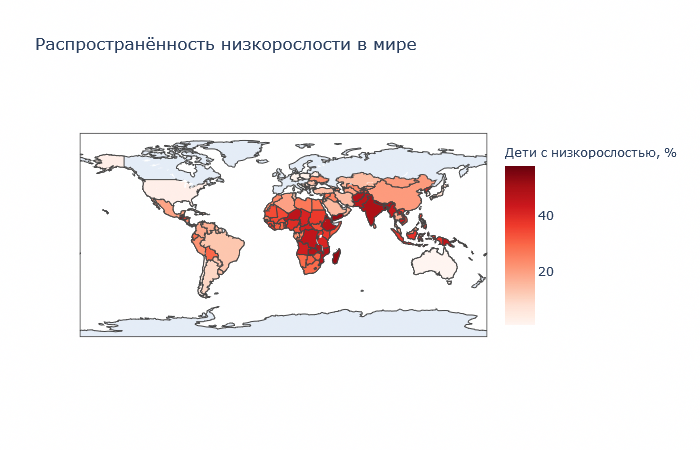
\includegraphics[width=125mm]{13.png}
\end{figure}


\end{frame}


\begin{frame}

\begin{figure}
	\centering
	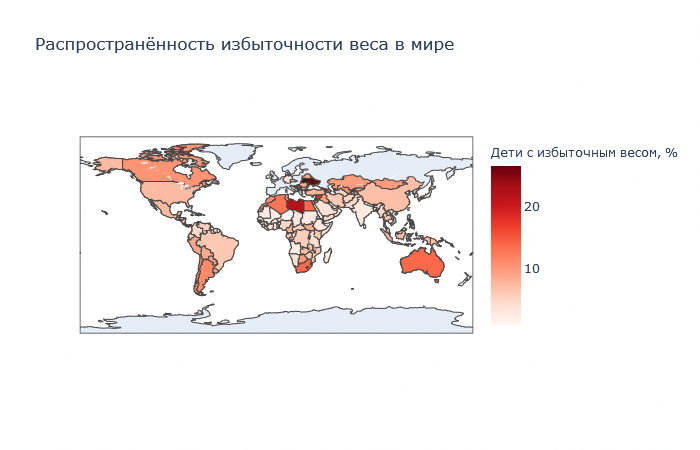
\includegraphics[width=125mm]{14.png}
\end{figure}


\end{frame}


\begin{frame}

\begin{figure}
	\centering
	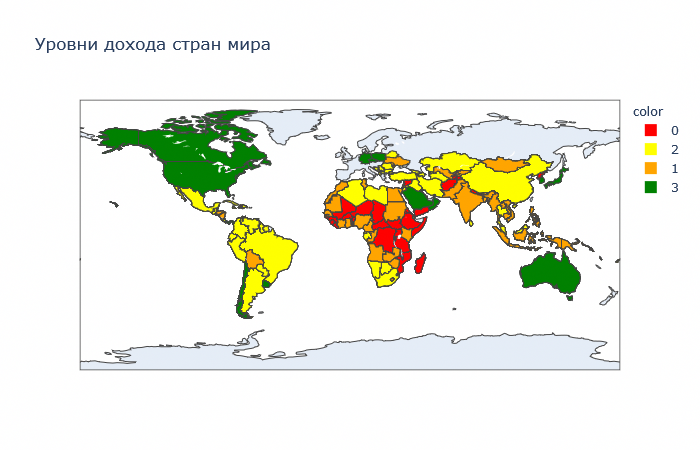
\includegraphics[width=120mm]{15.png}
\end{figure}


\end{frame}


\begin{frame}

\begin{figure}
	\centering
	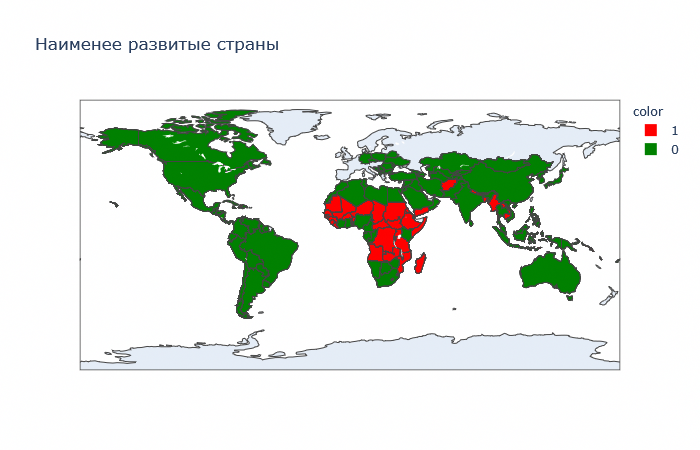
\includegraphics[width=120mm]{16.png}
\end{figure}


\end{frame}


\begin{frame}

\begin{figure}
	\centering
	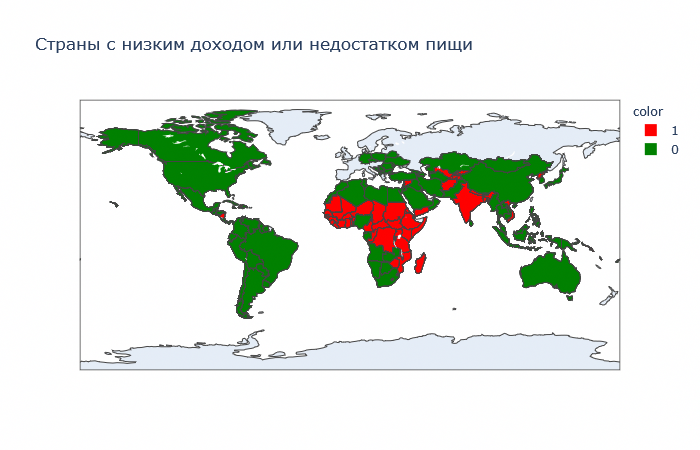
\includegraphics[width=120mm]{17.png}
\end{figure}


\end{frame}


\begin{frame}

\begin{figure}
	\centering
	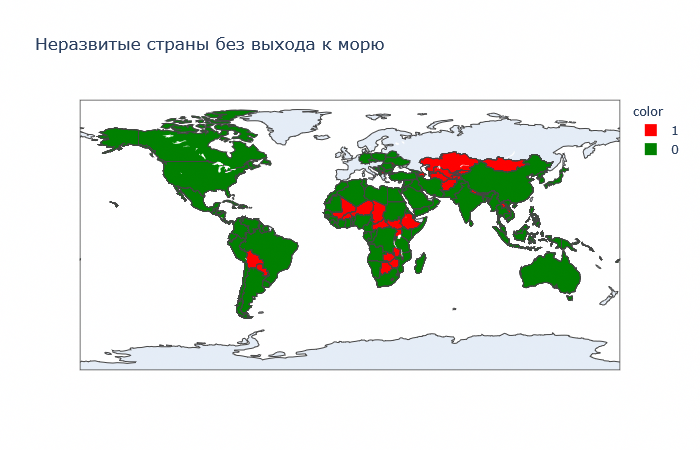
\includegraphics[width=120mm]{18.png}
\end{figure}


\end{frame}


\begin{frame}

\begin{figure}
	\centering
	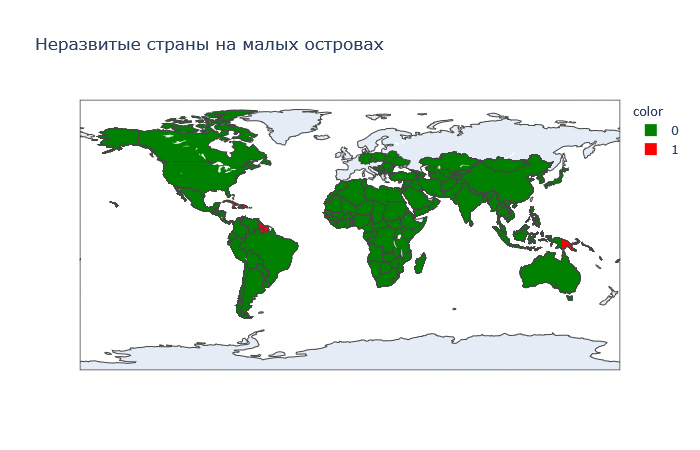
\includegraphics[width=120mm]{19.png}
\end{figure}


\end{frame}


\begin{frame}

\begin{figure}
	\centering
	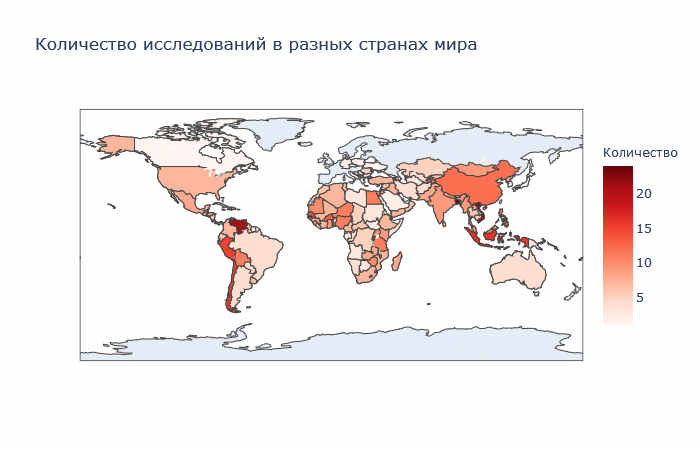
\includegraphics[width=125mm]{20.png}
\end{figure}


\end{frame}



\end{document}